
%%%%%%%%%%%%%%%%%%%%%%% file typeinst.tex %%%%%%%%%%%%%%%%%%%%%%%%%
%
% This is the LaTeX source for the instructions to authors using
% the LaTeX document class 'llncs.cls' for contributions to
% the Lecture Notes in Computer Sciences series.
% http://www.springer.com/lncs       Springer Heidelberg 2006/05/04
%
% It may be used as a template for your own input - copy it
% to a new file with a new name and use it as the basis
% for your article.
%
% NB: the document class 'llncs' has its own and detailed documentation, see
% ftp://ftp.springer.de/data/pubftp/pub/tex/latex/llncs/latex2e/llncsdoc.pdf
%
%%%%%%%%%%%%%%%%%%%%%%%%%%%%%%%%%%%%%%%%%%%%%%%%%%%%%%%%%%%%%%%%


\documentclass[runningheads,a4paper]{llncs}

\usepackage{amssymb}
\setcounter{tocdepth}{3}
\usepackage{graphicx}
\usepackage[hyphens]{url}
\usepackage{textcomp}
\usepackage{listings}
\lstset{
        basicstyle=\ttfamily\scriptsize,
        upquote=true,
        showspaces=false,
        showstringspaces=false,
        showtabs=false,
        tabsize=2,
        frame=none,
        breaklines,
        numbers=none,
        framexleftmargin=2mm,
        xleftmargin=2mm,
}

\usepackage{url}
\newcommand{\keywords}[1]{\par\addvspace\baselineskip
\noindent\keywordname\enspace\ignorespaces#1}

%% Define a new 'smallurl' style for the package that will use a smaller font.
\makeatletter
\def\url@smallurlstyle{%
  \@ifundefined{selectfont}{\def\UrlFont{\sf}}{\def\UrlFont{\scriptsize\ttfamily}}}
\makeatother
%% Now actually use the newly defined style.
\urlstyle{smallurl}
\newcommand{\nofootnote}[1]{~#1}

\begin{document}

\mainmatter  % start of an individual contribution

% first the title is needed
\title{A Tweet Consumer's Look At Twitter Through Linked Data Goggles Via Google Analytics}

% a short form should be given in case it is too long for the running head
\titlerunning{A Tweet Consumer's Look At Twitter}

% the name(s) of the author(s) follow(s) next
%
% NB: Chinese authors should write their first names(s) in front of
% their surnames. This ensures that the names appear correctly in
% the running heads and the author index.
%
\author{Thomas Steiner \and Arnaud Brousseau}
% the affiliations are given next; don't give your e-mail address
% unless you accept that it will be published
\institute{Google Germany GmbH, ABC-Str. 19, 20354 Hamburg, Germany\\
\url{{tomac|arnaudb}@google.com}}

%
% NB: a more complex sample for affiliations and the mapping to the
% corresponding authors can be found in the file "llncs.dem"
% (search for the string "\mainmatter" where a contribution starts).
% "llncs.dem" accompanies the document class "llncs.cls".
%


\maketitle

\begin{abstract}
Twitter Trends\footnote{\url{http://blog.twitter.com/2008/09/twitter-trends-tip.html}} allows for a global or local view on ``what's happening in my world right now" from a tweet producers' point of view. In this paper, we discuss the possibility to complete the functionality provided by Twitter Trends by having a closer look at the other side: the tweet consumers' -- i.e., readers' -- point of view. While Twitter Trends works by analyzing the frequency of terms and their velocity of appearence in tweets being written, our approach is based on the popularity of extracted named entities (in the sense of Linked Data) in tweets being read. Our experimentation architecture takes advantage of the possibility to use a client-side browser extension to harvest and dissect tweets from users' timelines, i.e., tweets supposed to be read. Named entities are extracted using several third-party Natural Language Processing (NLP) Web services in parallel, and are then reported to Google Analytics, which is used to store, analyze, and compute trends by pivoting Analytics data, e.g., users' geographic location, with the recorded named entities.
\end{abstract}

\section{Introduction}

\subsection{Twitter Trends}
http://blog.twitter.com/2010/12/to-trend-or-not-to-trend.html

\subsection{Google Chrome Extensions}
Google Chrome extensions\footnote{Google Chrome Extensions: \url{http://code.google.com/chrome/extensions/index.html}. Text adapted from the description to be found there.} are small software programs that can be installed to enrich the browsing experience with the Google Chrome browser. They are written using a combination of standard Web technologies, such as HTML, JavaScript, and CSS. Chrome extensions bundle all their files into a single file that gets usually (but not necessarily) distributed through the Chrome Web Store. There are several types of extensions, for this paper we focus on extensions based on so-called content scripts. Content scripts are JavaScript programs that run in the context of Web pages, similar to the Firefox Greasemonkey extension\footnote{Firefox Greasemonkey extension: \url{http://www.greasespot.net/}}. By using the standard Document Object Model (DOM), they can read or modify details of the Web pages a user visits. Examples of such modifications are, e.g., changing hyperlinks to remove potential @target="\_blank" attributes, or increasing the font size.

\subsection{Google Analytics}
 
\section{Twitter Swarm NLP Extension}
With our Twitter Swarm NLP extension\footnote{\url{https://chrome.google.com/webstore/detail/dpbphenfafkflfmdlanimlemacankjol}}, we inject JavaScript code via a content script into the Twitter.com homepage. The extension first checks if the user is logged in, and if so, retrieves the tweets of the logged-in user's timeline one-by-one, and performs NLP analysis via a remote NLP Web service on each of the tweets. The extracted entities are then displayed on the righthand-pane of the Twitter.com homepage, and sent to Google Analytics for further processing.

\subsection{Twitter Swarm NLP Web Service}
We have created a wrapper NLP Web service that merges results from existing third-party NLP Web services, namely from OpenCalais\footnote{\url{http://www.opencalais.com/}}, Zemanta\footnote{\url{http://www.opencalais.com/}}, AlchemyAPI\footnote{\url{http://www.alchemyapi.com/}}, and DBpedia Spotlight\footnote{\url{http://dbpedia.org/spotlight}}.
\subsection{Dealing With Extracted Entites On the Client Side}
\subsection{Dealing With Extracted Entites On the Google Analytics Side}

\begin{figure}[h!]
  \centering
  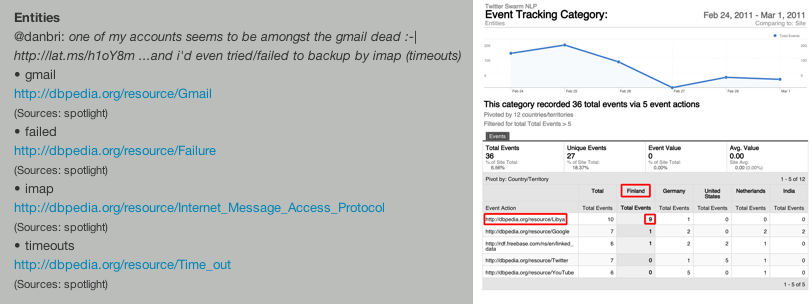
\includegraphics[width=0.95\linewidth]{combined.png}
  \caption{Left: Screenshot of the extracted entites of a particular tweet as displayed by the Twitter Swarm NLP Extension. Right: Test.}
  \label{fig:dataflow}
\end{figure}

\section{Related Work}

\subsection{Linked Open Social Signals (TWARQL)}
Previous work of Mendes et al.~\cite{Mendes:LOSS} have shown a possible implementation of real-time information both pushed and pulled from Twitter.
TWARQL\footnote{\url{http://wiki.knoesis.org/index.php/Twarql}} is based on a distributed architectures which features: 
\begin{itemize}
\item a client-side application which typically a Javacript-enabled web browser
\item a "Social Sensor Server" to receive tweets and filter them according to the user's request. It is worth noting here that TWARQL filtering is based on web-semantic technologies: SPARQL, hash-tag resolution through glossaries and LOD cloud are used to extract the highest amount of information possible from the Twitter Streaming API.
\item a number of distributed PuSH hubs which update clients as information flows (pushed-information model)
\item another server -- "Semantic Publisher" -- registers user's interest and updates the hubs. The updated information is eventually displayed on the user's screen.
\end{itemize}

\subsection{Twopular}

Twopular\footnote{Twopular website: \url{http://twopular.com/}} is a work of Martin Dudek. It aims at analysing current Twitter trends.
Since March 2008, Twopular takes advantage of OpenCalais services to extract entities from tweets retrieved from the Twitter Streaming API. \linebreak
Semantic entities are then used to reflect Twitter's current "trends".

\section{Conclusion}
Contributions: time filters (via Analytics), geographical pivoting (via Analytics)

As seen in the Related Work section, semantic analysis of a (real-time) Twitter stream is not new and has been successfully exploited to analyse tweets produced by the Twitter community.
What we propose here is an insight into tweets consumers' interests to provide a more accurate view of Twitter trends.

%%%%%%%%%%%%%%%%%%%%%%
%%%  Bibliography  %%%
%%%%%%%%%%%%%%%%%%%%%%

% The following two commands are all you need in the
% initial runs of your .tex file to
% produce the bibliography for the citations in your paper.
\bibliographystyle{abbrv}
\bibliography{typeinst}

\end{document}
